\section{Experimento - Detectando Robôs usando o Descritor HOG com o Clasificador SVM}
\label{HOG-SVM}

Sendo o algoritmo mais custoso computacionalmente, o reconhecimento de robôs roda com a resolução de 640x480 pixels e 15 quadros por segundo. O SVM foi treinado com um conjunto de imagens de pedestres humanos, os teste foram executados visando dois tipos de reconhecimento:
\begin{enumerate}
	\item SVM treinado com imagens humanas reconhecendo humanos- (Grupo de controle);
	\item SVM treinado com imagens humanas reconhecendo robôs;
	\item SVM treinado com imagens de robôs reconhecendo robôs.
\end{enumerate}


Para o descritor HOG um descritor padrão de 64x128 pixels foi usado da mesma forma que o artigo original, uma janela de 16x16 pixels, a célula que desliza pela imagem tem 32x32 pixels e um limiar de acerto de 0,5. Para o classificador SVM, o parâmetro de custo C ficou definido em 10 e o parâmetro $\Gamma$ ficou igual a 0.001, ambos escolhidos por uma busca em grade.

Como esperado, o classificador SVM, em conjunto com o descritor HOG, treinado com imagens de pessoas para reconhecimento de robôs é muito menos preciso do que o reconhecimento clássico de imagens de pessoas reconhecendo pessoas, entretanto, mesmo nessas circunstâncias, parece atingir a sua meta. Também foi reunida uma, mesmo que pequena, quantidade de imagens normalizadas contendo robôs, numa tentativa de verificar o quão bom esse algoritmo pode ser. Uma curva ROC foi plotada com as três situações, demonstrado na figura ~\ref{Fig:ROC} e o resultado de um quadro na figura ~\ref{Fig:Miltondet}:

\begin{figure}[!hH]
\centering
\includegraphics[width=12cm]{Imagens/ROC1.png}
\DeclareGraphicsExtensions.
\caption{Curvas ROC. A linha verde mostra o classificador clássico HOG-SVM, usado para reconhecimento de pessoas.
A linha vermelha demonstra o mesmo classificador treinado com pessoas usado para reconhecer robôs e a linha amarela mostra o classificador treinado com 100 imagens de robôs positivas e 100 imagens negativas usado na classificação dos robôs \\ Fonte: O Autor}
\label{Fig:ROC}
\end{figure}

As curvas ROC sugerem que o classificador treinado com imagens de robôs, mesmo com poucas imagens, parece ser, assintoticamente, melhor que a primeira abordagem usando o conjunto de imagens de pedestres. Nossa expectativa é fazer um classificador de robôs tão bom quanto o que reconhece pedestres. Devido a diversidade de robôs e sendo os seres humanos o nível máximo da forma humanoide, este classificador mostrou uma capacidade de generalização que poderia ser usada para reconhecer uma grande quantidade de robôs humanoides, dada uma quantidade suficiente de imagens de treinamento normalizadas.

\begin{figure}[!hH]
\centering
\includegraphics[width=7cm]{Imagens/Milton_Det.jpg}
\DeclareGraphicsExtensions.
\caption{Detecção do robô Milton usando imagens de pessoas como conjunto de treinamento. \\ Fonte: O Autor}
\label{Fig:Miltondet}
\end{figure} 

É possível ver que a cabeça do robô não foi incluída no retângulo de detecção, talvez, pela falta de imagens normalizadas de boa qualidade ou, talvez, pelo fato da cabeça não estar em conformidade com a cabeça humana
Como a aquisição de imagens tão específicas com uma mínima qualidade é de certa forma difícil de ser obter, a abordagem "Leave-One-Out" foi utilizada, já que lida bem com poucas amostras de treinamento.


\pagebreak

\section{Experimento - Detectando Robôs usando o Descritor HAAR com o Clasificador Boosting}
\label{HAAR-Boosting}
Uma limitação com relação à distância do robô a ser detectada foi inserida. No contexto atual da liga KidSize da RoboCup, outros robôs não têm a necessidade de serem detectados enquanto estiverem a mais de 3 metros de distância, devido a sua velocidade de andar ser bastante reduzida. 

Assim, A janela mínima de detecção foi definida com 150x150 pixels, ou seja, o menor objeto (robô) a ser detectado terá essa dimensão na imagem. O fato de limitar a janela de detecção mínima tem o principal objetivo de reduzir falsos positivos mas, também de acelerar o processo de detecção, já que menos janelas estarão contidas dentro da imagem. 

Durante o treinamento o número máximo de estágios foi determinado como sendo de 20 estágios, a taxa de acerto mínima foi configurada em 0.999, o parâmetro \(N_{\text{Pos}}\) após cálculo utilizando as equações ~\ref{eq1} e ~\ref{eq2} ficou fixada em 920, finalmente, a janela de amostragem foi de 150x150 pixels.

\begin{figure}[!hH]
    \centering
    \subfloat[]{{\includegraphics[width=4.5cm]{Imagens/Darwin01.png} }}
    \qquad
    \subfloat[]{{\includegraphics[width=4.5cm]{Imagens/Darwin02.png} }}
    \qquad
    \subfloat[]{{\includegraphics[width=4.5cm]{Imagens/Darwin03.png} }}
    \qquad
    \subfloat[]{{\includegraphics[width=4.5cm]{Imagens/Darwin04.png} }}
    \qquad
    \subfloat[]{{\includegraphics[width=4.5cm]{Imagens/Darwin05.png} }}
    \qquad
    \subfloat[]{{\includegraphics[width=4.5cm]{Imagens/Darwin06.png} }}
    \qquad
    \subfloat[]{{\includegraphics[width=4.5cm]{Imagens/Darwin07.png} }}
    \qquad
    \subfloat[]{{\includegraphics[width=4.5cm]{Imagens/Darwin08.png} }}
    \qquad
    \subfloat[]{{\includegraphics[width=4.5cm]{Imagens/Darwin09.png} }}
    \qquad
    \subfloat[]{{\includegraphics[width=4.5cm]{Imagens/Darwin10.png} }}
    \qquad
    \subfloat[]{{\includegraphics[width=4.5cm]{Imagens/Darwin11.png} }}
    \qquad
    \subfloat[]{{\includegraphics[width=4.5cm]{Imagens/Darwin12.png} }}

    \caption{Rastreamento do robô B2 usando características HAAR no campo de futebol com grama artificial.\\ Fonte: O Autor}
    \label{fig:Art}
\end{figure}


\begin{figure}[!hH]
\centering
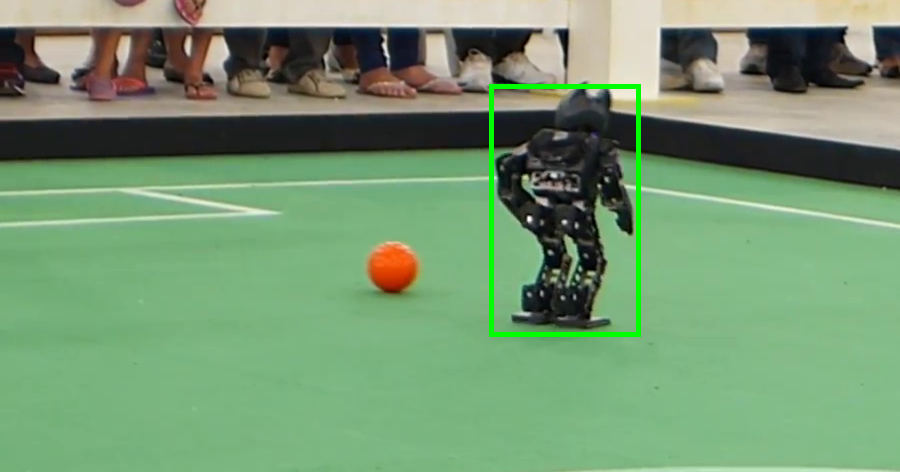
\includegraphics[width=8cm]{Imagens/HeartsHAAR.png}
\DeclareGraphicsExtensions.
\caption{Identificação do Robô Bold Hearts \cite{Bold} da universidade de Hertfordshire usando HAAR. \\ Fonte: Quadro extraído do video de qualificação do próprio time disponível no youtube.}
\label{fig_HeHAAR}
\end{figure}

\begin{figure}[!hH]
\centering
\includegraphics[width=8cm]{Imagens/HeartsHOG.png}
\DeclareGraphicsExtensions.
\caption{Identificação do Robô Bold Hearts \cite{Bold} da universidade de Hertfordshire usando HOG.\\ Fonte: Quadro extraído do video de qualificação do próprio time disponível no youtube.}
\label{fig_HeHOG}
\end{figure}


\section{Comparando os dois descritores e seus classificadores} 

O descritor HAAR teve um desempenho melhor que o descritor HOG em termos de velocidade, especialmente nas maiores resoluções. Entretanto quando o robô foi levado para o ambiente real, a iluminação se tornou um verdadeiro problema. Para ambos os algoritimos foi necessário incluir imagens negativas referentes ao ambiente. Na figura ~\ref{fig_rocHH} uma curva ROC que compara as capacidades e limitações dos dois algoritimos. 

\begin{figure}[!hH]
\centering
\includegraphics[width=12cm]{Imagens/ROCHH.png}\\
\DeclareGraphicsExtensions.
\caption{Curvas ROC. A linha verde mostra o algoritimo HOG-SVM clássico treinado com imagens de robôs usado para detecção de robôs.
A linha vermelha demonstra o resultado do classificador HAAR-AdaBoost treinado com o mesmo propósito.}
\label{fig_rocHH}
\end{figure}

As duas curvas ROC sugerem que os classificadores treinados parecem ser equivalentes. Devido à diversidade de robôs ambos os classificadores demonstraram capacidade de generalização que pode reconhecer diversos tipos de robôs dadas imagens de treinamento normalizadas suficientes.

Outro parâmetro de desempenho utilizado foi o de resposta dos algoritimos em quadros por segundo. É vital para um robô jogador de futebol que consiga detectar outros robôs em tempo real. A comparação desses parâmetros de desempenho estão na figura ~\ref{fig_fps}.

\begin{figure}[!hH]
\centering
\includegraphics[width=12cm]{Imagens/FPS.png}
\DeclareGraphicsExtensions.
\caption{Desempenho dos descritores HAAR-AdaBoost e HOG-SVM em termos de quadros por segundo após processamento. Esta informação é particularmente vital quando se trata de um robô que precisa agir rapidamente.\\ Fonte: O Autor}
\label{fig_fps}
\end{figure}

Os resultados mostram alguma vantagem para o HAAR-Adaboost em quadros por segundo, que pôde ser utlizado em full-hd 1920x1080 pixels mas, com alguns falso positivos, já que é uma técnica sensível à mudanças de iluminação. Já o HOG-SVM foi mais preciso em termos de detecção, porém com a limitação da taxa de velocidade e por consequência a resolução máxima de 640x480 pixels. Nas figuras ~\ref{fig:Mix1} e ~\ref{fig:Mix2} as mesmas imagens demonstrando as detecções para os dois algoritimos.

Aqui cabe uma ressalva, quando se trata de avaliar os descritores, os parâmetros escolhidos e o hardware foram verdadeiramente responsáveis pelo desempenho geral dos dois algoritimos.

O tempo gasto no treinamento e na normalização e redimensionamento das imagens tmabém foi uma questão complicada. Enquanto o HOG-SVM determinava todas as características por si só e levava no máximo 2 horas para efetuar o treinamento, o HAAR-Adaboost precisava que uma pessoa determinasse onde os objetos estavam em cada imagem positiva e seu treinamento levou de 5 a 12 horas para ser concluído. É válido lembrar que as imagens positivas do HOG-SVM precisaram ser redimensionadas o que levou um tempo considerável.


\begin{figure}[!hH]%
    \centering
    \subfloat[HOG - SVM]{{\includegraphics[width=10cm]{Imagens/MixHOG.png} }}%3.65
    \qquad
    \subfloat[HAAR - Boosting]{{\includegraphics[width=10cm]{Imagens/MixHAAR.png} }}%
    \caption{Vários robôs identificado usando o HOG-SVM e o HAAR-Boosting. Fonte: Quadro extraído do video de qualificação do time Bold Hearts - RoboCup 2015.}%
    \label{fig:Mix1}%
\end{figure}

\begin{figure}[!hH]%
    \centering
    \subfloat[HOG - SVM]{{\includegraphics[width=10cm]{Imagens/CIT01HOG.png} }}%3.65
    \qquad
    \subfloat[HAAR - Boosting]{{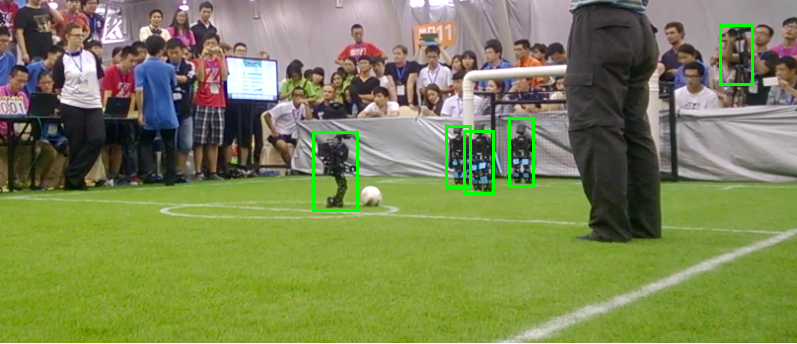
\includegraphics[width=10cm]{Imagens/CIT01HAAR.png} }}%
    \caption{Vários robôs identificado usando o HOG-SVM e o HAAR-Boosting. Fonte: O autor - RoboCup 2015.}%
    \label{fig:Mix2}%
\end{figure}

\pagebreak

